In game theory, the Nash equilibrium, named after the mathematician John Forbes Nash Jr., is a proposed solution of a non-cooperative game involving two or more players in which each player is assumed to know the equilibrium strategies of the other players, and no player has anything to gain by changing only their own strategy.
In terms of game theory, if each player has chosen a strategy, and no player can benefit by changing strategies while the other players keep theirs unchanged, then the current set of strategy choices and their corresponding payoffs constitutes a Nash equilibrium.

Stated simply, Alice and Bob are in Nash equilibrium if Alice is making the best decision she can, taking into account Bob's decision while his decision remains unchanged, and Bob is making the best decision he can, taking into account Alice's decision while her decision remains unchanged. Likewise, a group of players are in Nash equilibrium if each one is making the best decision possible, taking into account the decisions of the others in the game as long as the other parties' decisions remain unchanged. \\
\begin{figure}
    \centering
    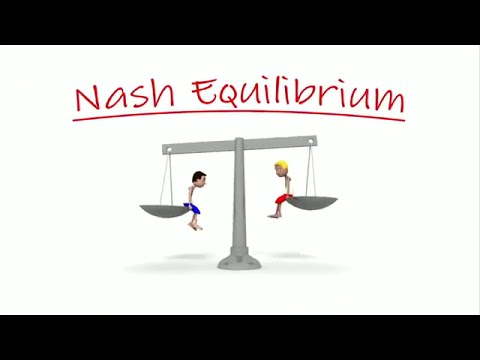
\includegraphics[]{equi.jpg}\\
    \caption{Nash}\\
    Source: https://i.ytimg.com/
    \label{game:3}
\end{figure}

Nash showed that there is a Nash equilibrium for every finite game
Game theorists use the Nash equilibrium concept to analyze the outcome of the strategic interaction of several decision makers. In other words, it provides a way of predicting what will happen if several people or several institutions are making decisions at the same time, and if the outcome for each of them depends on the decisions of the others. The simple insight underlying John Nash's idea is that one cannot predict the result of the choices of multiple decision makers if one analyzes those decisions in isolation. Instead, one must ask what each player would do, taking into account the decision-making of the others.